\documentclass[12pt,a4paper]{article}
%-------------------------------------------
%---Packages--------------------------------
%-------------------------------------------
\usepackage[utf8]{inputenc}
%\usepackage[T1]{fontenc}
%\usepackage{txfonts}
\usepackage{amsmath}
\usepackage{amsthm}
\usepackage{amsfonts}
\usepackage{array}
\usepackage{amssymb}
\usepackage{blindtext}
\usepackage{caption}
\usepackage{color}
\usepackage{csquotes}	    %
\usepackage{enumitem}	    %pour mieux bosser avec les listes. ajoute option label
\usepackage[yyyymmdd]{datetime}        %pour définir date custom
\usepackage{etaremune}
\usepackage{environ}
\usepackage{fancybox}
\usepackage{fancyhdr} 	    % Custom headers and footers
\usepackage{fancyref}
%\usepackage{float}
\usepackage{floatrow}       %float and floatrow can't be together...
\usepackage{gensymb}
\usepackage{graphicx}
\usepackage[colorlinks=true, linkcolor=purple, citecolor=cyan]{hyperref}
\usepackage{footnotebackref}
\usepackage{lipsum}
\usepackage{mathtools}
\usepackage{multicol}	    %gérer plusieurs colonnes
\usepackage{setspace}
\usepackage{subcaption}
\usepackage{todonotes}	    %Bonne gestion des TODOs
%TODO commenté pour tester l'utilité... à voir% \usepackage[tc]{titlepic}      %Permet de mettre une image en page de garde
\usepackage{tikz}	    % Pour outil de dessin puissant
\usepackage{ulem}	    %underline sur plusieurs lignes (avec \uline{})
\usepackage{vmargin} 	    %gestion des marges, avec dans l'ordre : gauche, haut, droit, bas, en-tête, entre en-tête et texte, bas de page, hauteur entre bas de page et texte
\usepackage{wrapfig}
\usepackage{xcolor}
\usepackage{xparse}                    %Pour utiliser NewDocumentCommand et des arguments 'mmooo'
%\usepackage{fullpage} 	    %supprime toutes les marges allouées aux notes, aussi en haut et en bas

%\ExplSyntaxOn
\pagestyle{fancyplain}	    %Makes all pages in the document conform to the custom headers and footers

%-------------------------------------------
%---Document Commands-----------------------
%---------------------------{----------------
\NewDocumentCommand{\framecolorbox}{oommm}
 {% #1 = width (optional)
  % #2 = inner alignment (optional)
  % #3 = frame color
  % #4 = background color
  % #5 = text
  \IfValueTF{#1}%
   {\IfValueTF{#2}%
    {\fcolorbox{#3}{#4}{\makebox[#1][#2]{#5}}}%
    {\fcolorbox{#3}{#4}{\makebox[#1]{#5}}}%
   }%
   {\fcolorbox{#3}{#4}{#5}}%
 }%
%------------------------------------------------
%------------------ENGLISH----------------------
%----------------------------------------------

\NewDocumentCommand{\epflTitle}{mO{Olivier Cloux}O{\today}O{Notes de Cours en}D<>{../../Common}}%Arguments : Matière, Auteur, Date, Titre du doc
{
\begin{titlepage}
    \vspace*{\fill}
    \begin{center}
        \normalfont \normalsize
        \textsc{Ecole Polytechnique Fédérale de Lausanne} \\ [25pt] % Your university, school and/or department name(s)
        \textsc{#4} %Titre du doc
        \\ [0.4 pt]
        \horrule{0.5pt} \\[0.4cm] % Thin top horizontal rule
        \huge #1 \\ % Matière
        \horrule{2pt} \\[0.5cm] % Thick bottom horizontal rule
        
\includegraphics[width=8cm]{#5/EPFL_logo}
        ~\\[0.5 cm]
        \small\textsc{#2}\\[0.4cm]
        \small\textsc{#3}\\
        ~\\
        ~\\
        
\includegraphics[scale=0.5]{#5/creativeCommons}
    \end{center}
    \vspace*{\fill}
\end{titlepage}
}


%-------------------------------------------
%-------------MATH NEW COMMANDS-------------
%-------------------------------------------
\newcommand{\somme}[2]{\ensuremath{\sum\limits_{#2}^{#1}}}
\newcommand{\produit}[2]{\ensuremath{\prod\limits_{#2}^{#1}}}
\newcommand{\limite}{\lim\limits_}
\newcommand{\llimite}[3]{\limite{\substack{#1 \\ #2}}\left(#3\right)}	%limites à deux condiitons
\newcommand{\et}{\mbox{ et }}
\newcommand{\deriv}[1]{\ensuremath{\, \mathrm d #1}}	%sigle dx, dt,dy... des dérivées/intégrales
%\newcommand{\fx}{\ensuremath{f'(\textbf{x}_0 + h}}
\newcommand{\ninf}{\ensuremath{n \to \infty}}	       %pour les limites : n tend vers l'infini
\newcommand{\xinf}{\ensuremath{x \to \infty}}	       %pour les limites : x tend vers l'infini
\newcommand{\infint}{\ensuremath{\int_{-\infty}^{\infty}}}
\newcommand{\xo}{\ensuremath{x \to 0}}									%x to 0
\newcommand{\no}{\ensuremath{n \to 0}}									%n zéro
\newcommand{\xx}{\ensuremath{x \to x}}									%x to x
\newcommand{\Xo}{\ensuremath{x_0}}										%x zéro
\newcommand{\X}{\ensuremath{\mathbf{X}} }
\newcommand{\A}{\ensuremath{\mathbf{A}} }
\newcommand{\R}{\ensuremath{\mathbb{R}} }								%ensemble de R
\newcommand{\rn}{\ensuremath{\mathbb{R}^n} } 							%ensemble de R de taille n
\newcommand{\Rm}{\ensuremath{\mathbb{R}^m} }  							%ensemble de R de taille m
\newcommand{\C}{\ensuremath{\mathbb{C}} }
\newcommand{\N}{\ensuremath{\mathbb{N}} }
\newcommand{\Z}{\ensuremath{\mathbb{Z}} }
\newcommand{\Q}{\ensuremath{\mathbb{Q}} }
\newcommand{\rtor}{\ensuremath{\R \to \R} }
\newcommand{\pour}{\mbox{ pour }}
\newcommand{\coss}[1]{\ensuremath{\cos\(#1\)}}						%cosinus avec des parenthèses de bonne taille (genre frac)
\newcommand{\sinn}[1]{\ensuremath{\sin\(#1\)}}					%sinus avec des parentèses de bonne taille (genre frac)
\newcommand{\txtfrac}[2]{\ensuremath{\frac{\text{#1}}{\text{#2}}}}		%Fractions composées de texte
\newcommand{\evalfrac}[3]{\ensuremath{\left.\frac{#1}{#2}\right|_{#3}}}
\renewcommand{\(}{\left(}												%Parenthèse gauche de taille adaptive
\renewcommand{\)}{\right)}
\newcommand{\longeq}{=\joinrel=}												%Parenthèse droite de taille adaptive


%-------------------------------------------------------
%------------------MISC NEW COMMANDS--------------------
%-------------------------------------------------------
\newcommand{\degre}{\ensuremath{^\circ}}
%\newdateformat{\eudate}{\THEYEAR-\twodigit{\THEMONTH}-\twodigit{\THEDAY}}



%-------------------------------------------------------
%------------------TEXT NEW COMMANDS--------------------
%-------------------------------------------------------
\newcommand{\ts}{\textsuperscript}
\newcommand{\evid}[1]{\textbf{\uline{#1}}}        %mise en évidence (gras + souligné)



%\newcommand{\Exemple}{\underline{Exemple}}
\newcommand{\Theoreme}{\underline{Théorème}}
\newcommand{\Remarque}{\underline{Remarque}}
\newcommand{\Definition}{\underline{Définition} }
\newcommand{\skinf}{\sum^{\infty}_{k=0}}
\newcommand{\combi}[2]{\ensuremath{\begin{pmatrix} #1 \\ #2 \end{pmatrix}}}	%combinaison parmi 1 de 2
\newcommand{\intx}[3]{\ensuremath{\int_{#1}^{#2} #3 \deriv{x}}}				%intégrale dx
\newcommand{\intt}[3]{\ensuremath{\int_{#1}^{#2} #3 \deriv{t}}}				%intégrale dy
\newcommand{\misenforme}{\begin{center} Mis en forme jusqu'ici\\ \line(1,0){400}\\ normalement juste, mais à améliorer depuis ici\end{center}}	%raccourci pour mise en forme
\newcommand*\circled[1]{\tikz[baseline=(char.base)]{
            \node[shape=circle,draw,inner sep=1pt] (char) {#1};}}			%pour entourer un chiffre
\newcommand{\horrule}[1]{\rule{\linewidth}{#1}} 				% Create horizontal rule command with 1 argument of height

\theoremstyle{definition}
\newtheorem{exemp}{Exemple}
\newtheorem{examp}{Example}


%-------------------------------------------
%---Environments----------------------------
%-------------------------------------------
\NewEnviron{boite}[1][0.9]{%
	\begin{center}
		\framecolorbox{red}{white}{%
			\begin{minipage}{#1\textwidth}
 	 			\BODY
			\end{minipage}
		}
	\end{center}
}
\NewEnviron{blackbox}[1][0.9]{%
	\begin{center}
		\framecolorbox{black}{white}{%
			\begin{minipage}{#1\textwidth}
 	 			\BODY
			\end{minipage}
		}
	\end{center}
}
\NewEnviron{exemple}[1][0.8]{%
    \begin{center}
        \framecolorbox{white}{gray!20}{%
            \begin{minipage}{#1\textwidth}
                \begin{exemp}
                    \BODY
                \end{exemp}
            \end{minipage}
        }
    \end{center}
}
\NewEnviron{suiteExemple}[1][0.8]{%
    \begin{center}
        \framecolorbox{white}{gray!20}{%
            \begin{minipage}{#1\textwidth}
                \BODY
            \end{minipage}
        }
    \end{center}
}
\NewEnviron{colExemple}[1][0.8]{%
    \begin{center}
        \framecolorbox{white}{gray!20}{%
            \begin{minipage}{#1\columnwidth}
                \begin{exemp}
                    \BODY
                \end{exemp}
            \end{minipage}
        }
    \end{center}
}
\NewEnviron{example}[1][0.8]{%
    \begin{center}
        \framecolorbox{white}{gray!20}{%
            \begin{minipage}{#1\textwidth}
                \begin{examp}
                    \BODY
                \end{examp}
            \end{minipage}
	}
    \end{center}
}
\NewEnviron{systeq}[1][l]{
			\begin{center}
				$\left\{\begin{array}{#1}
					\BODY
				\end{array}\right.$
			\end{center}
 }





%-------------------------------------------
%---General settings-----------------------
%-------------------------------------------
\renewcommand{\headrulewidth}{1pt}										%ligne au haut de chaque page
\renewcommand{\footrulewidth}{1pt}										%ligne au pied de chaque page
\setstretch{1.6}
\author{Olivier Cloux}

\usepackage[tc]{titlepic}
\usepackage{graphicx}
\usepackage{esint}
\usepackage{blindtext}
%\usepackage[a4paper]{geometry}
%\setcounter{section}{-1}
%\renewcommand{\contentsname}{Table des Matières}
\begin{document}
\setstretch{1}
\epflTitle{Physique 2}[Olivier Cloux][Fall 2015][Lectures Notes in]
\tableofcontents
\setstretch{1.6}
\section{Charge and Current}
We only will need 4 equations, the Maxwell's ones :
\begin{itemize}
	\item 	$\nabla \cdot \vec{E} = \frac{\rho}{\epsilon_0}$. $\vec{E}$ is the electric field. It means that "charge is the source of electric fields". Lectures 1-6
	\item	$\nabla \cdot \vec{B} = 0$. $\vec{B}$ is the magnetic fields. $\vec{B}$ fields have no beginning and no end. lectures 7-8
	\item $\nabla \times \vec{E} = -\frac{\delta \vec{B}}{\delta t}$. This is the induction. Lectures 9-10
	\item $\nabla \times \vec{B} = \mu_0 \vec{I} + \frac{1}{c^2}\frac{\delta\vec{E}}{\delta t}$. $\mu_0 \vec{I}$ this is the current (le courant) = the source of $\vec{B}$ Lectures 7-8. $\frac{1}{c^2}\frac{\delta\vec{E}}{\delta t}$ is the EM waves, on lectures 12.
\end{itemize}
\subsection{Electric Charge}
The reason hairs go away from the head with static electricity is because everything is positively charged, so hairs will go as far as possible of the head.

In a conductor, charges will clearly separate with each others, +/- in both side of the conductor. With an insulator, they will simply slightly separate.
\begin{boite}
	\evid{Definition} The amount of charge is conserved (never conserved), and is represented by Q (or q)
\end{boite}
When 2 objects differently charged touch each other, they will transfer charges until both are neutral.

By connecting two objects differently charged, + will go to - and this is Transient Current. With the same configuration, but with an object pushing current back to +, this is Steady Current

by definition, current is related with difference in charges : $I \iff \frac{\delta Q}{\delta t}$. So, current is \uline{exactly} defined by "moving charge". Exact same thing. Units and recap :
\begin{boite}
	\begin{center}
		\textbf{Current} is measured in \uline{Ampere [A]}\\
		\textbf{Charge} is measured in \uline{Coulomb [C]}
	\end{center}
	\begin{align*}
	I = \frac{\delta Q}{\delta t}\\
	Q = \intt{}{}{I(t)}
	\end{align*}
\end{boite}
\begin{example}
	Given a current $I(t) = 2-0.2t\ A$, how much charge passes in 5s ?
	\[Q = \int_0^5 2-0.2t \deriv{t}= \big[2t-0.1t^2\big]_0^5 = 10-2.5 = 5 C\]
\end{example}

\subsubsection{Point charge and charge densities}
\begin{boite}
	\evid{Definition :} Point charge : mathematical concept to simplify problems. We say that a charge Q is located on a point without spatial extension (this is not a single electron !)
\end{boite}
\textbf{Line charge density}
called $\lambda(L)$, for 1 dimension
\[Q = \int_L \lambda \deriv{L}\]
Used when only one coordinate is important. It does not mean that all charge is necessarily located on a line. It can also be used for wires and cylinders where for simplicity we can sometimes consider that all charge is located on a line in the centre.\\
\textbf{Surface charge density}
Called $\sigma(x,y)$, for 2 dimensions 
\[Q = \int\sigma(x,y)\deriv{x}\deriv{y} = \int \sigma(n)\deriv{n}\]
Used when two coordinates are important to describe the charge. This can be for example for a plane or the surface of a sphere or cylinder. In a practical sense this can often be used for metals because as we will see later all charge in that case is located on the surface.\\
\textbf{Volume charge density}
Called $\rho(x,y,z)$, for 3 dimensions
\[Q = \int_x \int_y \int_z \rho(x,y,z) \deriv{x}\deriv{y}\deriv{z} = \int_{\tau} \rho \deriv{\tau}\]
This is the most realistic situation where the amount of charge depends on three coordinates and it is therefore used for charged volumes. Also when no details are specified, such as for general laws, the volume charge density is used.

\subsection{Current as moving charges}
Let's consider 2 charged regions, one positively, one negatively. By connecting them, current will flow, heating the wire and creating what we call \textbf{current}. After a while, both sides are neutral. This is \textit{transient current}. If we keep adding negative (or positive) charges to a side, the current won't stop, and we speak of a \textit{steady current}.

\subsubsection{current density}
A few paragraphs ago, we defined charge density. If we can do it with charges, we can easily do it with current too. We thereby define \textbf{current density $\vec{j}$} ; we can restrict ourselves to \textit{volume current density}, as we'll almost never encounter surface or linear current density.

Given a surface, we define a small surface $\deriv{A}$, and the vector normal to this area $ \deriv{\vec{A}}$. $\vec{J}$ can be expressed as the current per unit area normal to the flow

We know that
\[dI = \vec{J}\cdot d\vec{A}\]
Thus, there are 2 possibilities : either $d\vec{A} \perp \vec{J} \to dI = 0$ or $d\vec{A} \parallel \vec{J} \to dI = \max$

We can then calculate :
\[I = \int_A \vec{J}\cdot d\vec{A},\quad	\(= \int_A JdA\cos\theta\)\]


\section{Coulomb's law}

\subsection{Derivation on Coulomb's law}
Coulomb's law represents the law of force between charges (in vacuum). In order to understand Coulomb force and how it was derived in the eighteenth century, we have to explain 3 aspects first :

\evid{Direction :} 	From Newton's first law, we know that for every action there is an equal and opposite action. Thus, the force of charge 1 on charge 2 is the opposite (yet equal) of the force of charge 2 on charge 1 :
\[\vec{F}_{12} =-\vec{F}_{21}\]
This means that the Coulomb's force is a \textit{central force}.

\evid{Dependence on \textit{magnitude} and \textit{sign} of charges :} Earlier, we proved that equal charges repel each others, when opposite charges tend to attract. Mathematically, this can be represented with signed multiplication : equal signs give positive sign, when opposite signs give a negative sign. We also saw that the force increases when at least one of the charges increase, which is comparable to multiplication too. We can then imagine :
\[F \propto Q_1Q_2\]

\evid{Dependence on distance}
Thanks to Coulomb (and a much more elegant experience of Cavendish), we can say that :
\[F \propto \frac{1}{r^2}\]
In the International Unit System, the proportionality constant is 
\[\frac{1}{4\pi\epsilon_0} \simeq 9\times 10^9 Nm^2C^{-2}[mF^{-1}]\]
Also, $\epsilon_0$ is the \textit{permittivity of free space}\footnote{sometimes called the dielectric constant} and is defined as 
\[\epsilon_0 \simeq 8.8\times 10^{-12}Fm^{-1}\]

\begin{boite}
	\evid{Coulomb's law}	
	\begin{align*}
		\vec{F} = \frac{1}{4\pi\epsilon_0} \frac{Q_1Q_2}{r_{12}^2}\text{\^{r}}_{12}
	\end{align*}
	And the unit vector between $Q_1$ and $Q_2$ :
	\[\text{\^{r}}_{12} = \frac{\vec{r}_{12}}{|r_{12}|}\]
\end{boite}

\misenforme

\subsection{Example of the long rode}
\[F = \frac{Q\lambda L}{4\pi\epsilon_0\sqrt{x^2 + \(\frac{L}{2}\)^2}}\]

\section{Week 3 : Electric fields}
Definition of a field :
\[\vec{E} = \frac{\vec{F}}{Q_t}\]
Force of a field is determined by the density of field lines. Direction of the lines indicate the direction of the field. 
\subsection{Finding the E-field due to charges}
\evid{Single point charge} 
\[\vec{E} = \frac{Q}{4\pi\epsilon_0 r^2}\text{\^{r}} \(\simeq \frac{\vec{F}(Q_t)}{Q_t}\)\]
\evid{For a collection of point charges}... simply the sum of all points.\\

\subsection{Electric potential}
$W_{AB}$ work to bring a charge from a to b.\\
$Q_t$ a test charge.
$V_{AB}$ potential difference between a and b.\\
Potential of point charge :
\[\vec{E} = \frac{Q\text{\^{r}}}{4\pi\epsilon_0 r^2} \quad V_P = \int_\infty^P -\frac{Q\text{\^{r}} \cdot\deriv{\vec{L}}}{4\pi\epsilon_0 r^2}\]

\subsection{Charge in E-fields}
Assumption : Q has no influence on E-field (Q small and E kept constant) 
\[\vec{F} = Q\vec{E} = m\vec{a}\]
\begin{align*}
	u_B - u_A = Q(v_B-v_A) = -\int_A^B \vec{E} \cdot \deriv{\vec{r}} = \int_B^A Q E \deriv{x}  \int_B^A ma\deriv{x} \\
	\text{as }a = v\frac{\deriv{v}}{\deriv{s}}\\
	= \int_B^A mv \deriv{v} = \text{velocity !}\\
	\to Q(v_B - v_A) = \frac{1}{2}mv_A^2 - \frac{1}{2}mv_B^2 = \Delta E_{kin}
\end{align*}
So : E-field accelerates charges !



\section{Gauss, Poisson, Laplace}
If a solution can be found, it's the only one possible.

\section{Capacitance and dielectrics}
\begin{boite}
	The capacity is the amount of charge a conductor can hold for a given potential "capacity of charge", and is defined by 
	\[C = \frac{Q}{V}\]
	in $CV^{-1}$ or $F$ (Farad). C only depends on geometry. \\
	Let's note too $V = \frac{Q}{4\pi \epsilon r_0} \to$
	\begin{boite}[0.3]
		\[C = 4\pi\epsilon r_0\]
	\end{boite}
	Which is valid for any sphere. Also :
	\[\Delta V = \frac{Q}{C}\]
\end{boite}

\subsection{Parallel plate capacitor}
$\sigma$ = surface charge density = $\frac{Q}{A}$, $E = \frac{\sigma}{\epsilon_0} = \frac{Q}{\epsilon A} \to \Delta V = Ed = \frac{Qd}{\epsilon A} \to C = \frac{Q}{V} = \epsilon\frac{A}{d}$

\subsection{Polarization of matter}
Very interesting for industry. Much possibility, very money.
so manly

\subsection{Gauss's law with dielectrics}
\[\oiint_S \vec{E}\cdot \deriv{\vec{S}}= \sum_i \frac{Q_i}{\epsilon_0}\]
\section{}
\section{}
\subsection{}
\subsection{}
\subsection{Combinations of B- and E-fields}
\begin{boite}
	E field determines \textbf{kinetic energy}\\
	B-field determines \textbf{momentum}\\
	E- and B-field together determine velocity
\end{boite}
\subsection{Magnetic dipole}
Dipole moment $\vec{m}$ = $I\vec{A} \quad (IA\vec{e_n})$. The torque : $\vec{T} = \vec{m} \times \vec{B}$
\subsubsection{Magnetic field due to magnetic dipole}
$E_r = \frac{2p\cos\theta}{4\pi\epsilon_0 r^3}$
\subsection{}
\subsection[Mag. dipole : and. momentum, precession]{Magnetic dipole in B-field : angular momentum and precession}
All magnetic dipoles also have angular momentum $\vec{L}$\\
Main requirement for precession : $\vec{T} \perp \vec{L}$

Electrical dipole will have no momentum, and no procession. Magnetic dipole will have both.

\subsection*{Magnetic flux}
Similar to flux of E-field :
\begin{equation}
	\Phi = \int_A \vec{B} \cdot \deriv{\vec{A}}
\end{equation}

\subsection*{Using magnetic flux to find force and torque on a large circuit}
Potential energy per small loop : $\deriv{U} = -\vec{m} \cdot \vec{B}$

\subsection{Summary: elements in and as sources of B-field}
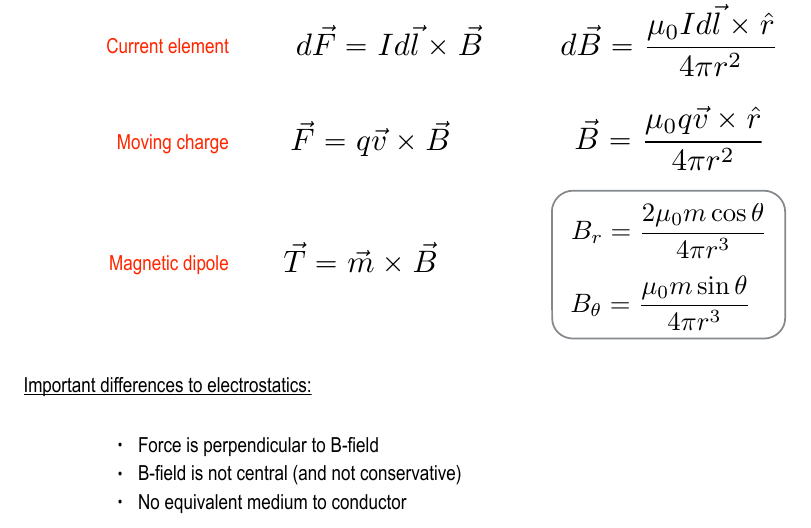
\includegraphics[scale=0.7]{images/summary_b-field}

\subsection*{Gauss' law for B-fields}
General case :
\begin{equation}
	\oiint_S \vec{B} \cdot \deriv{\vec{S}} = 0
\end{equation}




\begin{boite}
	\evid{Lorentz Force} : 
	\[\vec{F} = q\vec{v}\times \vec{B}\]
\end{boite}



\section{Recap}
\subsection{Glossary}
\begin{itemize}
	\item $\vec{E}$ : \textbf{Electric field}
	\item $\vec{B}$ : \textbf{Magnetic field}
	\item $\lambda$ : \textbf{Line charge density} : $\frac{Q}{L}$
	\item $\sigma$ : \textbf{Surface charge density} : $\frac{Q}{A}$
	\item $\rho$ : \textbf{Volume charge density} : $\frac{Q}{V}$
	\item $\deriv{A}$ : an infinitesimally small part of an \textbf{open surface}
	\item $\deriv{S}$ : an infinitesimally small part of a \textbf{close surface} (those 2 are not fixed, just typically used for that).
	\item $\epsilon$ : the permittivity of free space
	\item $\chi_e$ : \textbf{Electric susceptibility}. How easy it is to polarise a material. A constant, one per material.	
	\item $\vec{J}$ : \textbf{current density} at a point (verify that !)
\end{itemize}

\subsection{Equations}
\begin{itemize}
	\item 	Relationship between current and charges : $I = \frac{\deriv{Q}}{\deriv{t}} \iff Q = \int I(t) \deriv{t}$
	\item 	Force between two charges : \textbf{Coulomb's law} : $\vec{F} = \frac{1}{4\pi\epsilon_0}\frac{Q_1Q_2}{r_{12}^2}\hat{r}_{12}$
\end{itemize}

\subsection{Values}
\begin{itemize}
	\item 	An electron's charge : $1.6\times 10^{-19} C$
	\item 	An electron's mass : $9.1 \times 10^{-31} kg$	
	\item 	$\epsilon_0 \simeq 8.8\times 10^{-12}Fm^{-1}$
	\item 	$\frac{1}{4\pi\epsilon_0} \simeq 9\times 10^9 Nm^2C^{-2}[mF^{-1}]$
\end{itemize}































\end{document}  